\documentclass[电力电子]{subfiles}
\begin{document}
\section{画图题}
\begin{ti}[10 分]
	单相桥式全控整流电路接电阻负载。$\alpha = 60^\circ$,画出输出电压 $u_{\dd}$ 和电流 $i_{\dd}$ 的波形。
\end{ti}

\begin{ti}[10 分]
	下图所示为单相全桥电压型逆变电路,试画出输出电压 $u_{\oo}$ 和输出电流 $i_{\oo}$ 的波形。
\end{ti}

\begin{ti}[10 分]
	单相桥式全控整流电路接阻感负载。$\alpha = 30^\circ$,画出输出电压 $u_{\dd}$ 和 $i_{\dd}$ 的波形。
\end{ti}

\begin{ti}[10 分]
	在三相半波整流电路中,$\alpha = 0^\circ$,试绘出在电阻性负载整流电压 $u_{\dd}$ 和电流 $i_{\dd}$ 的波形。
\end{ti}

\begin{ti}[10 分]
	如图所示为一降压斩波电路,试画出输出电压 $u_{\oo}$ 和输出电流 $i_{\oo}$ 的波形(电流断续)。
\end{ti}

\begin{ti}[10 分]
	在三相半波整流电路中,$\alpha = 60^\circ$,如果 a 相的触发脉冲消失,试绘出在电阻性负载整流电压 $u_{\dd}$ 的波形和晶闸管 V1 的电压 $u_{\text{V1}}$ 的波形。
\end{ti}

\begin{ti}[10 分]
	单相桥式全控整流电路接电阻负载。$\alpha = 60^\circ$,画出输出电压 $u_{\dd}$ 和电流 $i_{\dd}$ 的波形。
\end{ti}

\begin{ti}[10 分]
	三相全控桥整流电路,带阻感负载,$L$ 值极大,电阻 $R =$ \SI{5}{\Omega},变压器二次相电压为 \SI{200}{V},控制角 $\alpha = 60^\circ$,试回答:画出整流输出电压 $u_{\dd}$ 的波形,画出晶闸管 \V 的电压 $u_{\V}$ 的波形。
\end{ti}

\begin{ti}[10 分]
	在三相半波整流电路中,$\alpha = 60^\circ$,试绘出在电阻性负载整流电压 $u_{\dd}$ 和电流 $i_{\dd}$ 的波形。
\end{ti}

\begin{ti}[10 分]
	三相全控桥整流电路,带阻感负载,$L$ 值极大,电阻 $R =$ \SI{5}{\Omega},变压器二次相电压为 \SI{200}{V},控制角 $\alpha = 90^\circ$,试回答:画出整流输出电压 $u_{\dd}$ 的波形,画出晶闸管 \V 的电压 $u_{\V}$ 的波形。
\end{ti}

\begin{ti}[10 分]
	在三相半波整流电路中,$\alpha = 90^\circ$,试绘出在电阻性负载整流电压 $u_{\dd}$ 和电流 $i_{\dd}$ 的波形。
\end{ti}

\begin{ti}[10 分]
	三相全控桥整流电路,带阻感负载,$L$ 值极大,电阻 $R =$ \SI{5}{\Omega},变压器二次相电压为 \SI{200}{V},控制角 $\alpha = 30^\circ$,试回答:画出整流输出电压 $u_{\dd}$ 的波形,画出晶闸管 \V 的电压 $u_{\V}$ 的波形。
\end{ti}

\begin{ti}[10 分]
	在三相半波整流电路中,$\alpha = 60^\circ$,如果 a 相的触发脉冲消失,试绘出在电阻性负载整流电压 $u_{\dd}$ 的波形和晶闸管 V\textsubscript{1} 的电压 $u_{\text{V\textsubscript{1}}}$ 的波形。
\end{ti}

\begin{ti}[10 分]
	画出电阻负载单相交流调压电路的输出电压波形和晶闸管承受的电压波形。
\end{ti}

\begin{ti}[5 分]
	单相桥式半控整流电路接电阻负载。$\alpha = 30^\circ$,画出输出电压 $u_{\dd}$ 的波形。
\end{ti}

\begin{ti}[10 分]
	如图所示为一降压斩波电路,试画出输出电压 $u_{\oo}$ 和输出电流 $i_{\oo}$ 的波形。
\end{ti}

\begin{ti}[10 分]
	单相半波可控整流电路接阻感负载。$\alpha = 30^\circ$,画出输出电压 $u_{\dd}$ 和电流 $i_{\dd}$ 压波形。
\end{ti}

\begin{ti}[10 分]
	画出升降压斩波电路的原理图和电流波形图(电流连续)。
\end{ti}

\begin{ti}[10 分]
	三相全控桥整流电路,带阻感负载,$L$ 值极大,控制角 $\alpha = 60^\circ$,试画出整流输出电压 $u_{\dd}$ 的波形,画出晶闸管 \V 的电压 $u_{\V}$ 的波形。
\end{ti}

\begin{ti}[10 分]
	画出降压斩波电路图,分别画出 V 在开通和关断状态的等效电路图。
\end{ti}

\begin{ti}[10 分]
	三相全控桥整流电路,带电阻负载,控制角 $\alpha = 0^\circ$,试画出整流输出电压 $u_{\dd}$ 的波形,画出晶闸管 \V 的电压 $u_{\V}$ 的波形。
\end{ti}

\begin{ti}[10 分]
	画出由 IGBT 组成的单相桥式逆变电路带阻感性负载的电路图。
\end{ti}

\begin{ti}[5 分]
	画出三相桥式逆变电路图。
\end{ti}

\begin{ti}[10 分]
	三相全控桥整流电路,带阻感负载,$L$ 值极大,控制角 $\alpha = 90^\circ$,试画出整流输出电压 $u_{\dd}$ 波形,画出晶闸管 \V 的电压 $u_{\V}$ 的波形。
\end{ti}

\begin{ti}[10 分]
	在三相半波整流电路中,$\alpha = 60^\circ$,如果 a 相的触发脉冲消失,试绘出在电阻性负载整流电压 $u_{\dd}$ 的波形和晶闸管 V1 的电压 $u_{\mathrm{V}1}$ 的波形。
\end{ti}

\begin{ti}[10 分]
	IGBT 电压型单相桥式逆变电路及栅极驱动信号波形如图所示,试对应驱动信号画出输出电压 $u_{\oo}$ 及负载电流 $i_{\oo}$ 的波形。
	\begin{center}
		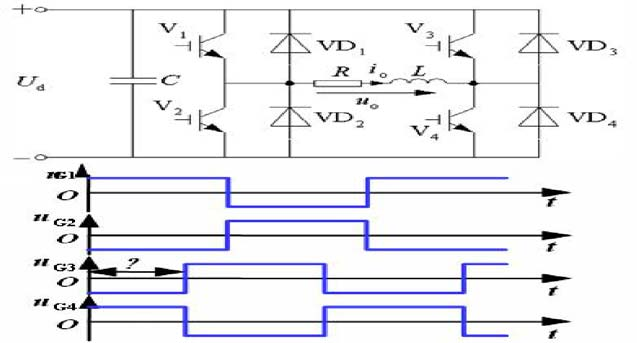
\includegraphics[width=0.6\textwidth]{figure/fig6}
	\end{center}
\end{ti}

\begin{ti}[10 分]
	三相全控桥整流电路,带阻感负载,$L$ 值极大,控制角 $\alpha = 30^\circ$,试画出整流输出电压 $u_{\dd}$ 的波形,画出晶闸管 \V 的电压 $u_{\V}$ 的波形。
\end{ti}

\begin{ti}[10 分]
	画出由 IGBT 组成的单相桥式带阻感性负载的变流电路图。
\end{ti}

\begin{ti}[5 分]
	在三相桥式全控整流电路中,电阻负载,假设 VT\textsubscript{1} 不能导通,画出 $\alpha = 0^\circ$ 整流电压 $u_{\dd}$ 波形。
\end{ti}

\begin{ti}[15 分]
	三相桥式全控整流电路,带电阻电感负载,$L$ 值极大,当 $\alpha = 60^\circ$ 时,要求:画出 $u_{\dd}$、$i_{\dd}$ 和 $i_{\mathrm{VT_{1}}}$ 的波形。
\end{ti}

\begin{ti}[10 分]
	单相桥全控整流电路带电阻负载 $\alpha = 30^\circ$ 时,画出 $u_{\dd}$ 及 $u_{\mathrm{VT}_{1}}$ 的波形。
\end{ti}

\begin{ti}[10 分]
	画出单相交流调压电路 $\alpha = 30^\circ$ 时,$u_{\oo}$ 及 $u_{\mathrm{VT}}$ 的电压波形。
\end{ti}

\begin{ti}[10 分]
	单相桥式全控整流电路接电感负载。$\alpha = 60^\circ$,画出输出电压 $u_{\dd}$ 和电流 $i_{\dd}$ 的波形。
\end{ti}

\begin{ti}[10 分]
	分别画三相半波整流电路电感性负载 $\alpha = 60^\circ$ 和三相全控有源逆变电路电感性负载 $\beta = 30^\circ$ 的输出电压 $u_{\dd}$ 波形。
\end{ti}

\begin{ti}[10 分]
	分别画三相半波整流电路电感性负载 $\alpha = 0^\circ$ 和三相全控有源逆变电路电感性负载 $\beta = 30^\circ$ 的输出电压 $u_{\dd}$ 波形。
\end{ti}

\begin{ti}[10 分]
	单相半波可控整流电路接电阻负载。$\alpha = 30^\circ$,画出输出电压 $u_{\dd}$ 和晶闸管承受的电压 $u_{\mathrm{VT}}$ 波形。
\end{ti}

\begin{ti}[10 分]
	三相全控桥整流电路,带电阻负载,画出 $\alpha = 60^\circ$ 整流输出电压 $u_{\dd}$ 的波形,画出晶闸管 VT\textsubscript{1} 的电压 $u_{\mathrm{VT}_{1}}$ 的波形。
\end{ti}

\begin{ti}[10 分]
	单相半波可控整流电路接阻感负载。$\alpha = 30^\circ$,画出输出电压 $u_{\dd}$ 和晶闸管承受的电压 $u_{\mathrm{VT}}$ 波形。
\end{ti}

\begin{ti}[10 分]
	画出降压斩波电路的原理图和输出电压电流波形图(电流连续)。
\end{ti}

\begin{ti}[10 分]
	单相半波可控整流电路接阻感负载。$\alpha = 30^\circ$,画出输出电压 $u_{\dd}$ 和电流 $i_{\dd}$ 压波形。
\end{ti}

\begin{ti}[10 分]
	三相全控桥整流电路,带电阻负载,画出 $\alpha = 90^\circ$ 整流输出电压 $u_{\dd}$ 的波形,画出晶闸管 VT\textsubscript{1} 的电流 $i_{\mathrm{VT}_{1}}$ 的波形。
\end{ti}
\end{document}